\begin{appendix}
\chapter{Anhang}
\label{chap:anhang}

\section{Flächenflugzeug}
\label{sec:herleitung_geschw_bez}
Der in Gleichung \ref{eq:geschw_flaechenflugzeug} aufgeführte Zusammenhang entsteht aus dem Verhältnis der Fluggeschwindigkeiten bei konstanten Auftriebsbeiwert. Aus der Definition des Auftriebsbeiwertes
\begin{equation}
	c_{A} = \frac{A}{\rho/2\cdot V^2\cdot S}
\end{equation}
entsteht durch Umformen die Beziehung für die Geschwindigkeit
\begin{equation}
	V = \sqrt{\frac{2\cdot A}{\rho\cdot S \cdot c_{A}}} \eqend{.}
\end{equation}
Im Horizontalflug (\ensuremath{\gamma = 0}) kompensiert der Auftrieb lediglich die Gewichtskraft (Vgl. Gleichung \ref{eq:auftriebsgleichung_vereinfacht})
\begin{equation}
	A = G \eqend{.}
\end{equation}
Für jegliche Art von Steigflug (\ensuremath{\gamma \neq 0}) ist dies nicht mehr der Fall. Unter der Voraussetzung einer gleichen Gewichtskraft \ensuremath{m\cdot g}, gleicher Flügelfläche \ensuremath{S} und einem konstanten Auftriebsbeiwerts \ensuremath{c_{A}} ergibt sich für das Verhältnis der Geschwindigkeiten \ensuremath{V/V^\star}
\begin{equation}
	\frac{V}{V^\star} = \frac{\sqrt{\frac{2\cdot m \cdot g\cdot \cos\gamma}{\rho\cdot S \cdot c_{A}}}}{\sqrt{\frac{2\cdot m\cdot g}{\rho^\star \cdot S \cdot c_{A}}}} = \sqrt{\cos\gamma\cdot\frac{\rho^\star}{\rho}} \eqend{.}
\end{equation}\\

\section{Propeller}
\label{sec:propellerkennfeld}
In Abb. \ref{abb:propellerkennfeld} ist ein Kennfeld von einem APC 10x3 Propeller dargestellt. 
\begin{figure}[H]
\centering
	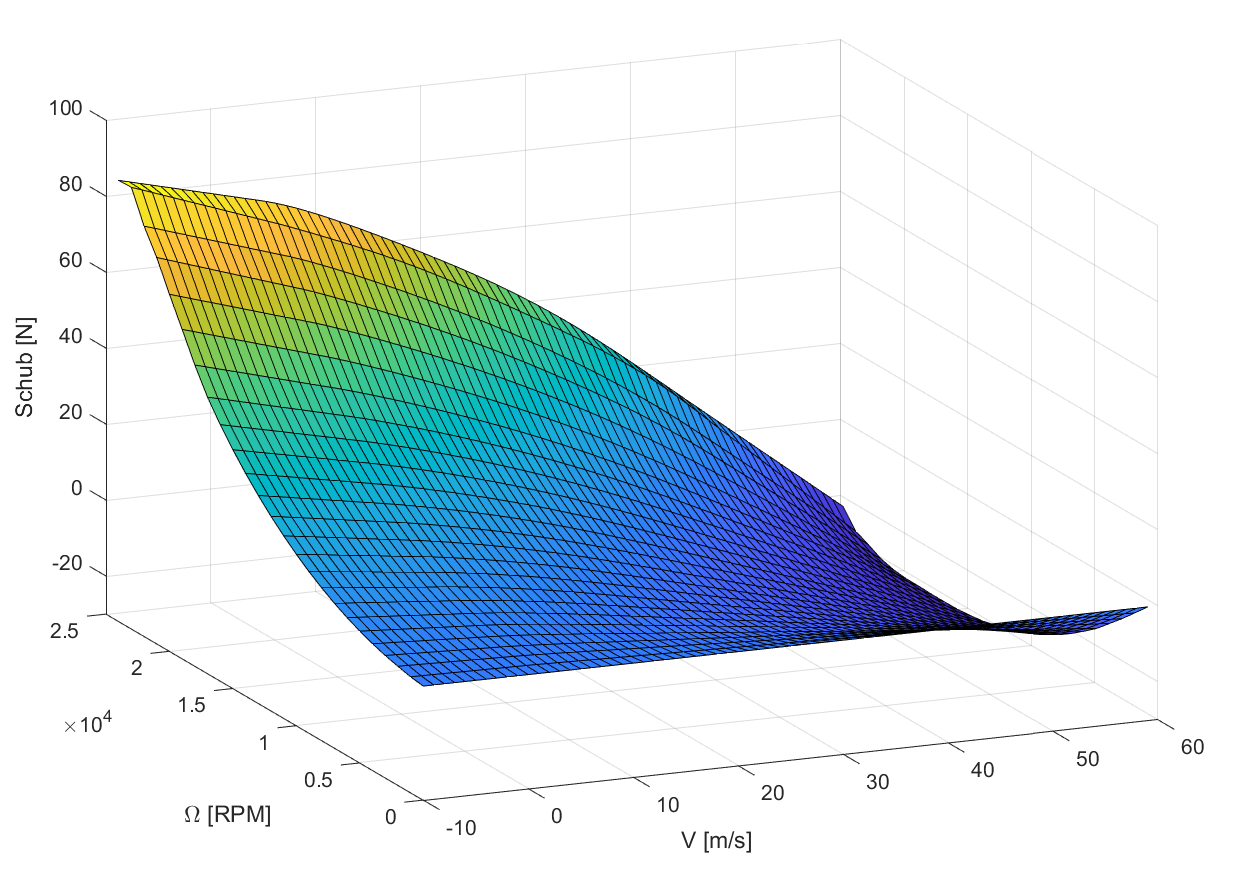
\includegraphics[scale=0.7]{Diagramme/Propellerkennfeld.pdf}
	\caption{beispielhaftes Propellerkennfeld für einen APC 10x3 Propeller}
	\label{abb:propellerkennfeld}
\end{figure}

\section{Motor}
\label{sec:motormodell}
Das Motormodell weist eine über das ganze Spektrum der möglichen Betriebspunkte konsistente Verteilung des Motorwirkungsgrades auf (Vgl. Abb. \ref{abb:motormodell}). Der maximale Motorwirkungsgrad wird bei maximaler Spannung und bei maximalen Strom erreicht. Der errechnete Wert stimmt mit einer Genauigkeit von \ensuremath{\pm \SI{2}{\%}} mit den Angaben vom Hersteller überein \cite{axi}.
\missingfigure{2D Darstellungen des Motormodells}
\begin{figure}[H]
\centering
	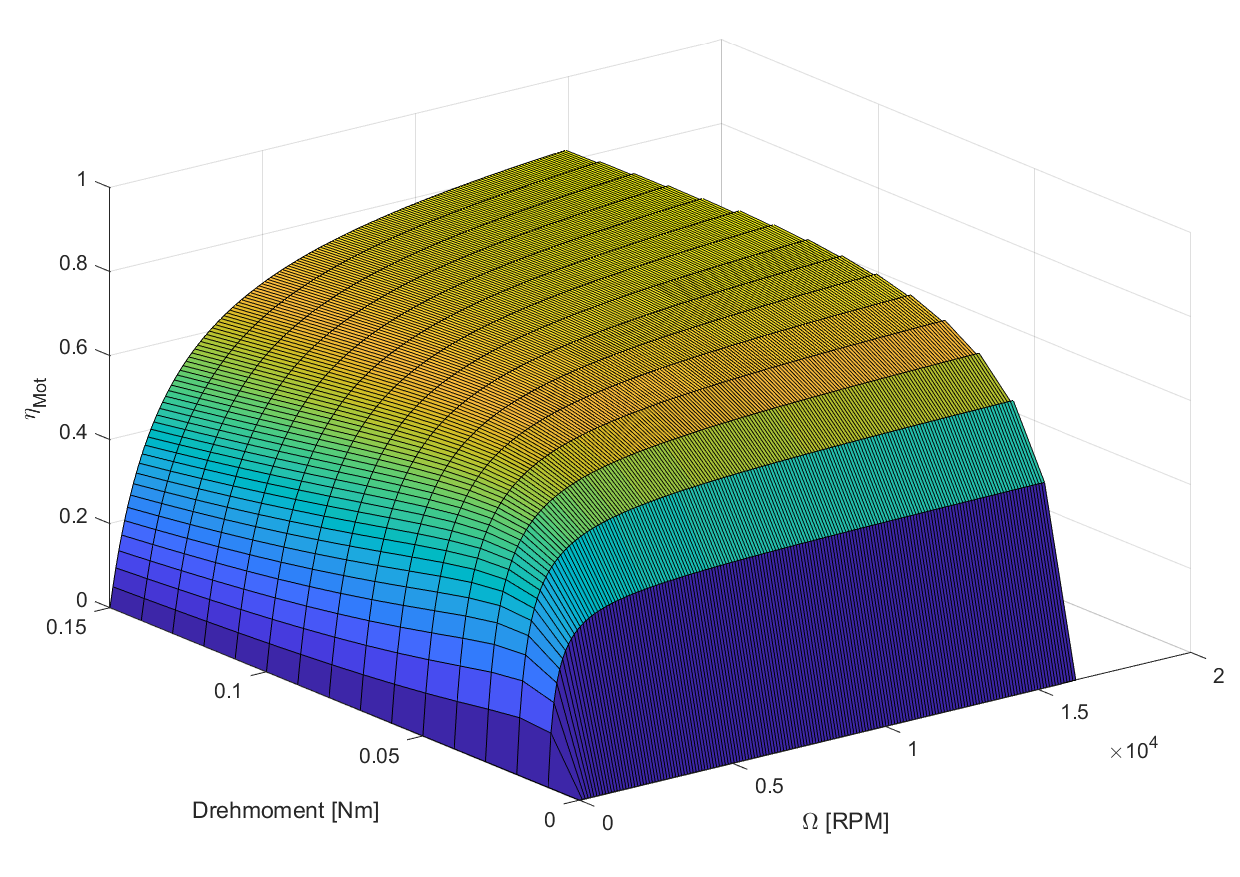
\includegraphics[scale=0.7]{Diagramme/Motormodell.pdf}
	\caption{Wirkungsgrad aufgetragen über verschiedenen Betriebspunkten des Motors}
	\label{abb:motormodell}
\end{figure}

\section{Batteriekapazität}
Für die Untersuchungen ist eine Berechnung der Batteriekapazität unabhängig von der Art der Zelle, aber abhängig von der Batteriemasse von Interesse.
Aus diesem Grund bietet sich die Energiedichte an. 
Mit dieser berechnet sich die Kapazität wie folgt:
\begin{equation}
	C_{Bat}	= \omega\cdot\frac{m_{Bat}}{U_{Bat,nom}} \eqend{.}
	\label{eq:batteriekapazitaet}
\end{equation}


\section{Vergleich von normierter zur originalen Batteriezelle}
\label{sec:norm_vs_orig}
Für den Vergleich der Norm- mit der Originalzelle wird das Integral unterhalb der beiden Entladekurven für eine bestimmte Entladerate gebildet. Anschließend werden beide Flächen zu einander in Beziehung gesetzt 
\begin{equation}
	\text{Toleranz} = \frac{\text{F}_{Orig.}-\text{F}_{Norm}}{\text{F}_{Norm}} \eqend{.}
\end{equation} 
Im Sinne einer Genauigkeitssteigerung werden alle die Batterien in der Normzellenberechnung nicht berücksichtigt, deren individuelle Abweichung eine große Diskrepanz zur Standardabweichung aufweist. Der Vergleich zeigt, dass es starke Abweichungen der Batterie gibt. Die durchschnittliche Abweichung liegt für Entladeraten bis \SI{45}{1/h} deutlich über Null und steigt mit der Entladerate von \SI{8}{\%} auf \SI{17}{\%} bei \SI{45}{1/h}. Die Spannung der Normzelle ist somit im Durchschnitt kleiner als die der originalen Batteriezelle (Vgl. Abb. \ref{abb:batterie_abweichungen}). Ab der Entladerate von \SI{50}{1/h} fällt die Abweichung drastisch auf \SI{-18}{\%} ab. 
\begin{figure}[H]
\centering
	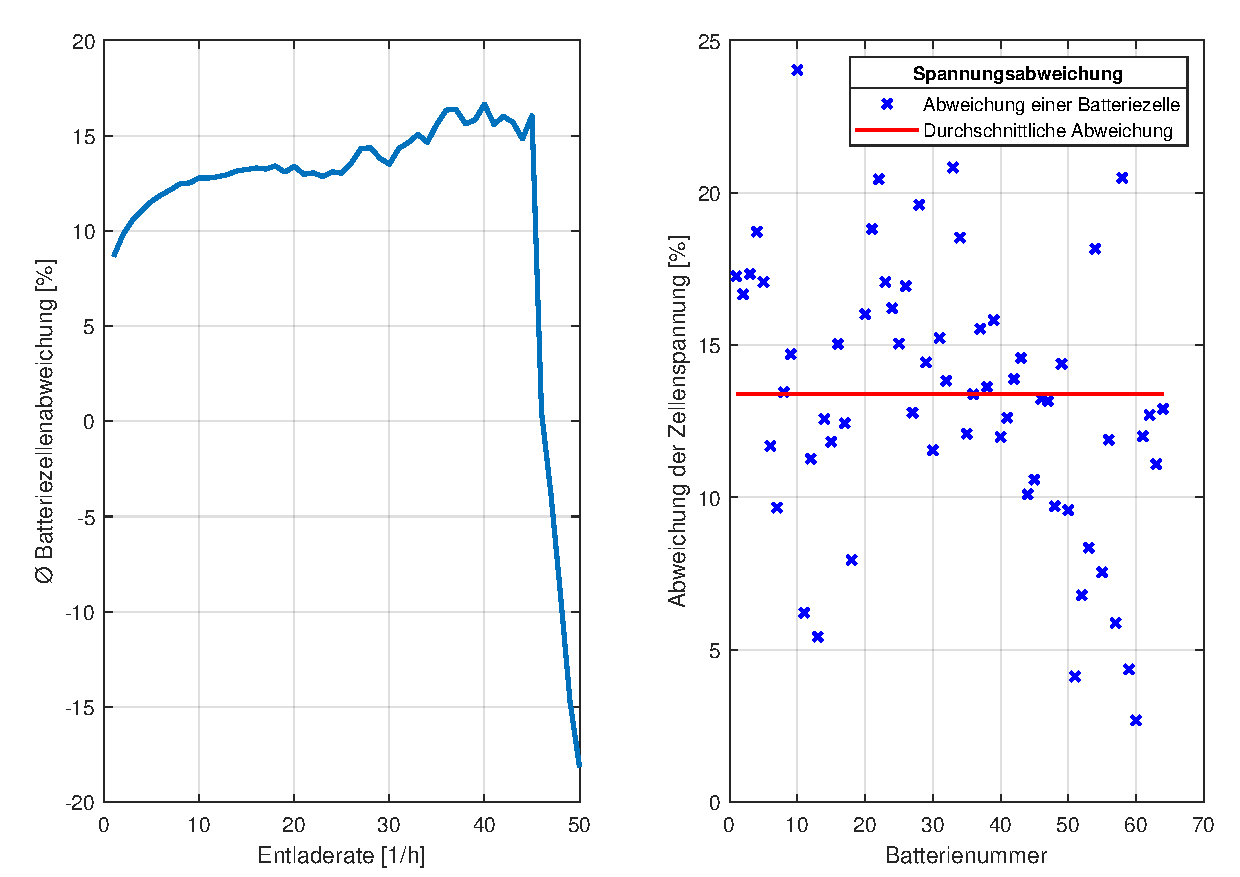
\includegraphics[scale=0.7]{Diagramme/Abweichungen.pdf}
	\caption{links: Durschnittliche Spannungsabweichungen der Normzelle von den Zellen aus der Batteriedatenbank in Abhängigkeit von der C-Rate,\\ rechts: Beispiel für die Spannungsabweichungen jeder Normzelle im Vergleich zur Originalzelle für eine Entladerate von \SI{20}{1/h}
	 }
	\label{abb:batterie_abweichungen}
\end{figure}


\section{Steiggeschwindigkeit}
\label{sec:vvar_vorgehen}
\begin{center}
\begin{figure}[H]
\begin{struktogramm}(163,160)
\while[5]{Für alle Bahngeschwindigkeiten}
	\assign[2]{Berechne Gesamtmasse}
	\assign[2]{Flugzeit für Höhenschritt berechnen}			
	\while[5]{Solange Abbruchkriterium nicht erreicht}
		\assign{Aerodynamik berechnen}
	\whileend
	\assign[2]{Schub berechnen}
	\assign[2]{Schub auf Propeller verteilen}
	\ifthenelse[10]{1}{4}{Schub zu gro\ss{}?}{ja}{nein}
		\assign[2]{Ergebnis verwerfen (NaN)}
		\change
		\assign[2]{Drehzahl und Drehmoment aus Propellerkennfeld interpolieren}
		\assign[2]{Motorzustand berechnen}
		\assign[2]{Zustand der Motorregler berechnen}
		\assign[2]{Zustand der Batterie neu berechnen}
		\assign[2]{Gesamtwirkungsgrad berechnen}
	\ifend
	\ifthenelse[10]{1}{1}{Werden Grenzen überschritten?}{ja}{nein}
		\assign[2]{Ergebnis verwerfen (NaN)}
		\change
		\assign[2]{Ergebnis beibehalten}
	\ifend
	\assign[2]{Speichern der aufgebrachten Energiemenge}
\whileend
\ifthenelse[10]{5}{1}{Sind die Werte NaN?}{nein}{ja}
	\while[5]{Solange Abbruchkriterium nicht erreicht}		
		\assign[2]{Finde den Index mit der geringsten verbrauchten Energiemenge}
		\ifthenelse[10]{1}{3}{Werte innerhalb Leistungsgrenzen?}{ja}{nein}
			\assign[2]{Verlasse Schleife}
			\change
			\assign[2]{Suche nächst kleinere Energiemenge}
		\ifend
	\whileend
	\assign[2]{Übergabe aller Leistungsparameter mit diesem Index}
		\change
	\assign[2]{Verwerfe alle Ergebnisse}
\ifend
\end{struktogramm}
\caption{Programmstruktur zur Ermittlung der optimalen Steiggeschwindigkeit}
\label{abb:steiggeschw}
\end{figure}
\end{center}

\section{Motorreglerwirkungsgrad}
\label{sec:motorreglerwirkungsgrad}
Im Folgenden ist der Einfluss des ESC-Wirkungsgrades auf den TOC veranschaulicht. Dafür werden zwei Batteriegrößen untersucht, eine mit sechs Zellen und einmal mit acht Zellen. Die Masse und Kapazität bleiben jeweils gleich. 

\begin{figure}[H]
\centering
	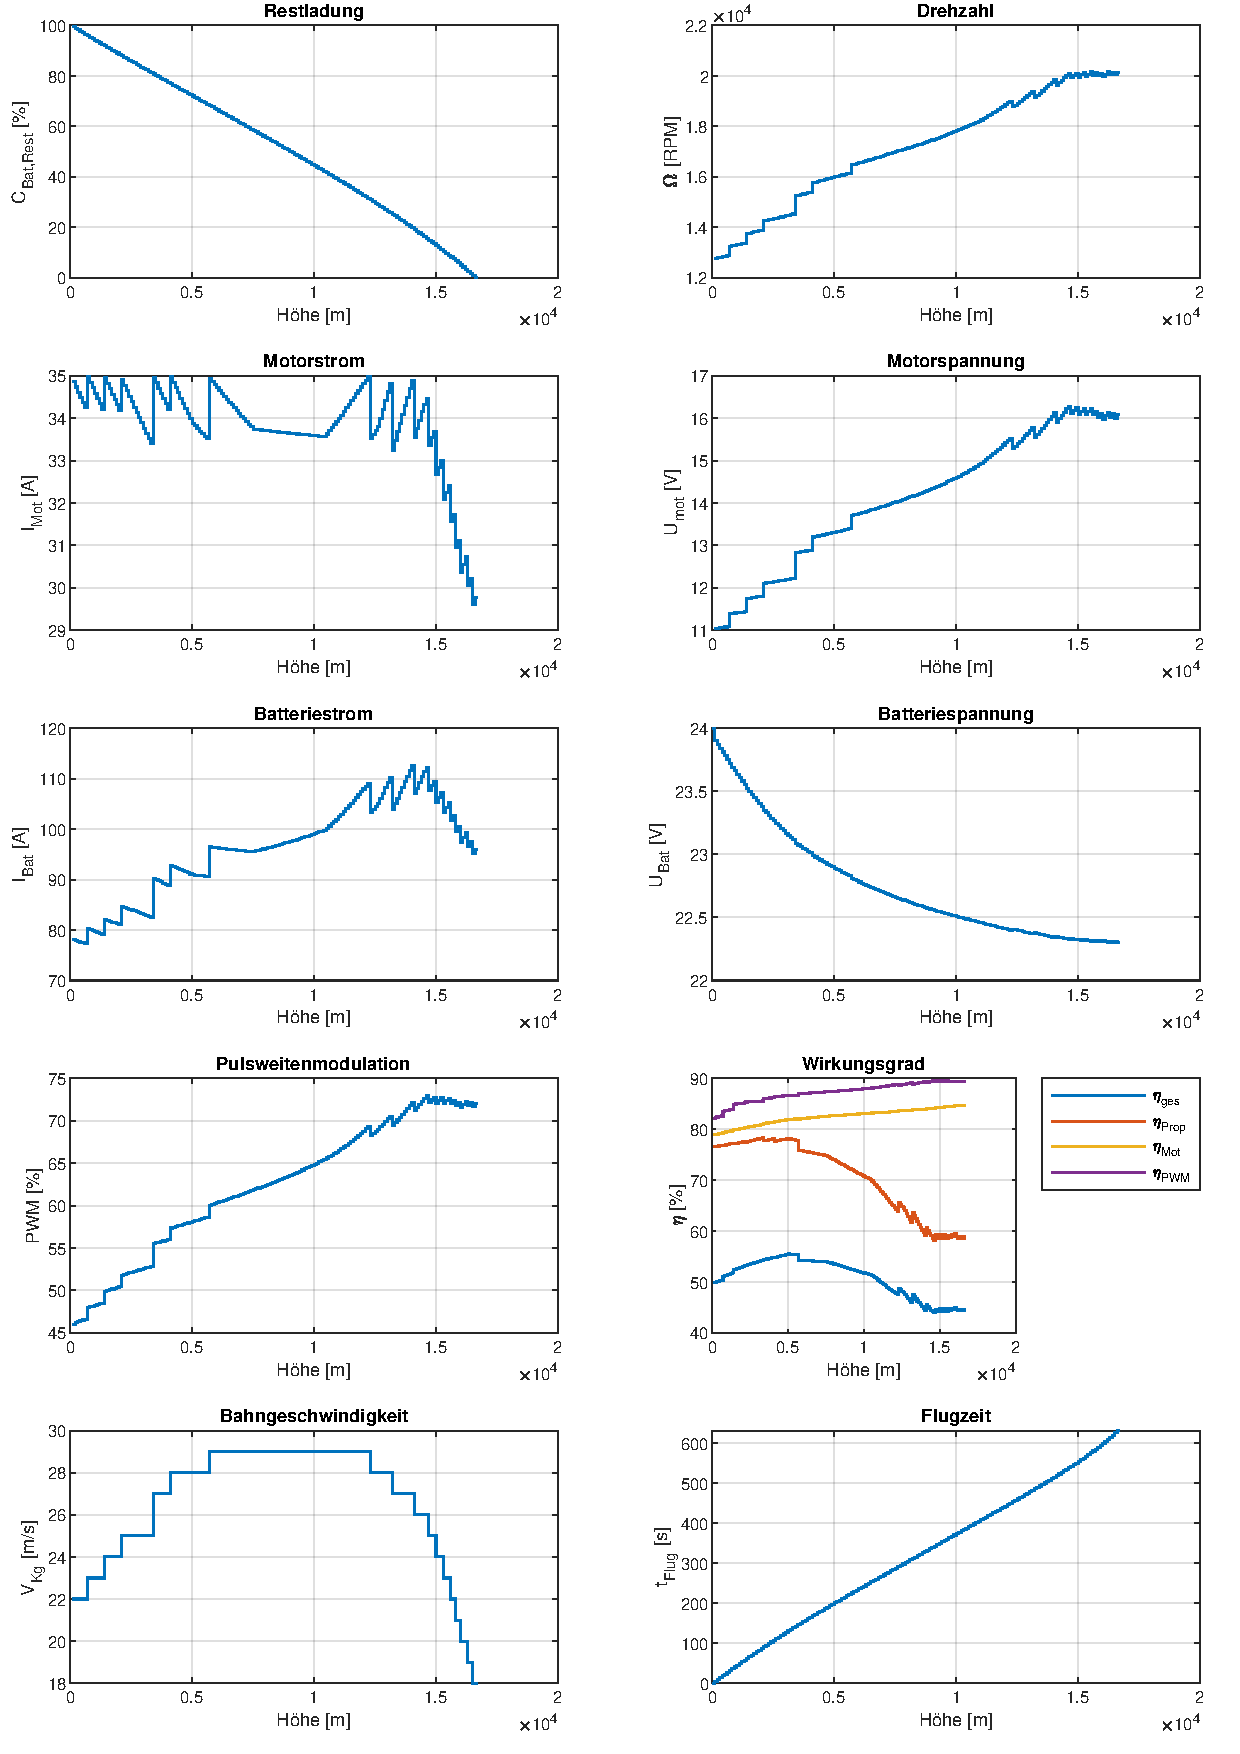
\includegraphics[scale=0.7]{Diagramme/Untersuchung_eta_pwm_normal_6.pdf}
	\caption{Leistungsparameter für einer Verbesserung des Motorreglerwirkungsgrades (Halbierung der Verluste) für eine Batterie mit sechs Zellen}
	\label{abb:eta_pwm_6_normal}
\end{figure}

\begin{figure}[H]
\centering
	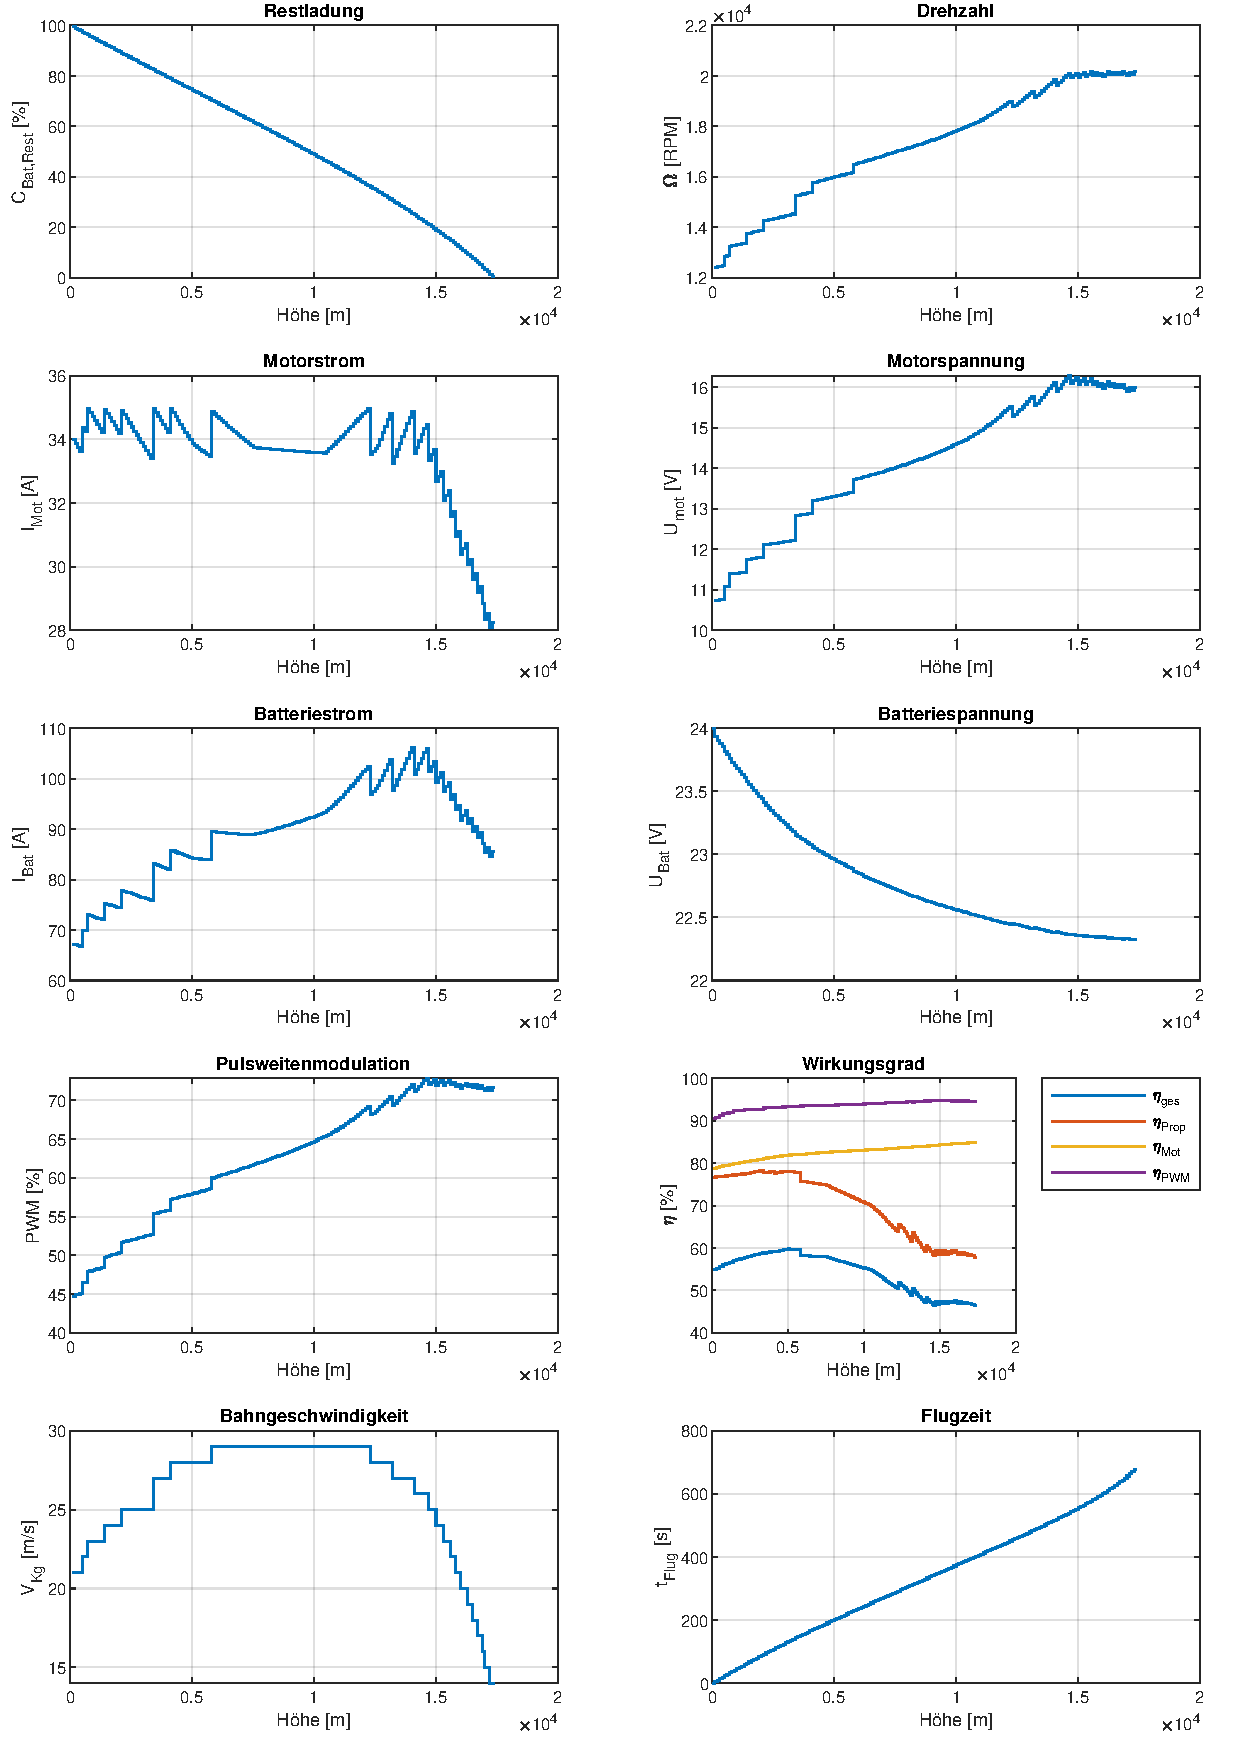
\includegraphics[scale=0.7]{Diagramme/Untersuchung_eta_pwm_halbierung_6.pdf}
	\caption{Leistungsparameter für einer Verbesserung des Motorreglerwirkungsgrades (Halbierung der Verluste) für eine Batterie mit sechs Zellen}
	\label{abb:eta_pwm_6_halb}
\end{figure}

\begin{figure}[H]
\centering
	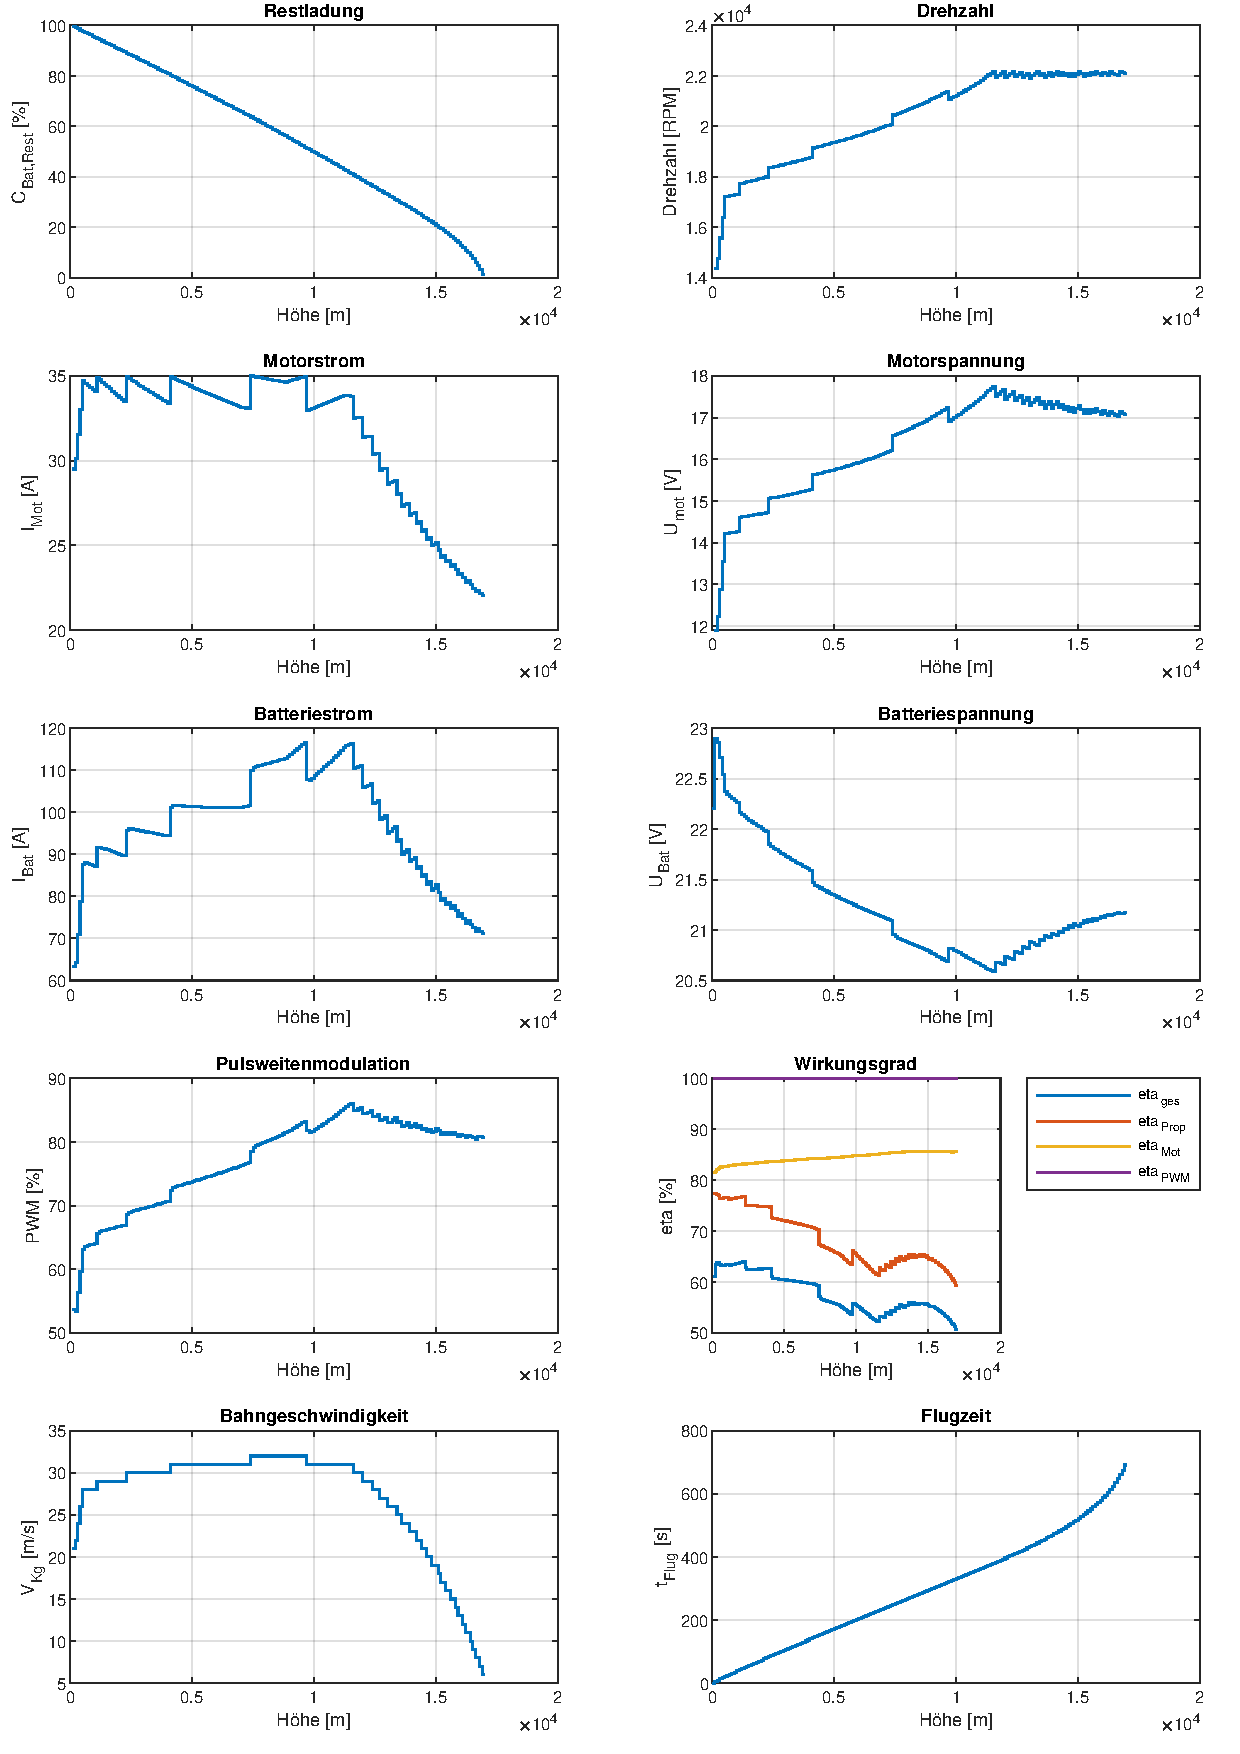
\includegraphics[scale=0.7]{Diagramme/Untersuchung_eta_pwm_1_6.pdf}
	\caption{Leistungsparameter für einer Verbesserung des Motorreglerwirkungsgrades (keine Verluste) für eine Batterie mit sechs Zellen}
	\label{abb:eta_pwm_6_1}
\end{figure}


\section{Batteriemasse}
Es zeigt sich, dass das Optimum des Batteriemassenanteils bei \SI{66.66}{\%} oder leicht darunter liegt. Eine Erhöhung führt zu schlechteren Flugleistungen und einem schnelleren Absinken der Restkapazität gegen Null. Deutlich ist zudem der Einfluss der Batteriemasse auf die Bahngeschwindigkeit gegeben. Mit der Masse sinkt die optimale Bahngeschwindigkeit. 
\begin{figure}[H]
\centering
	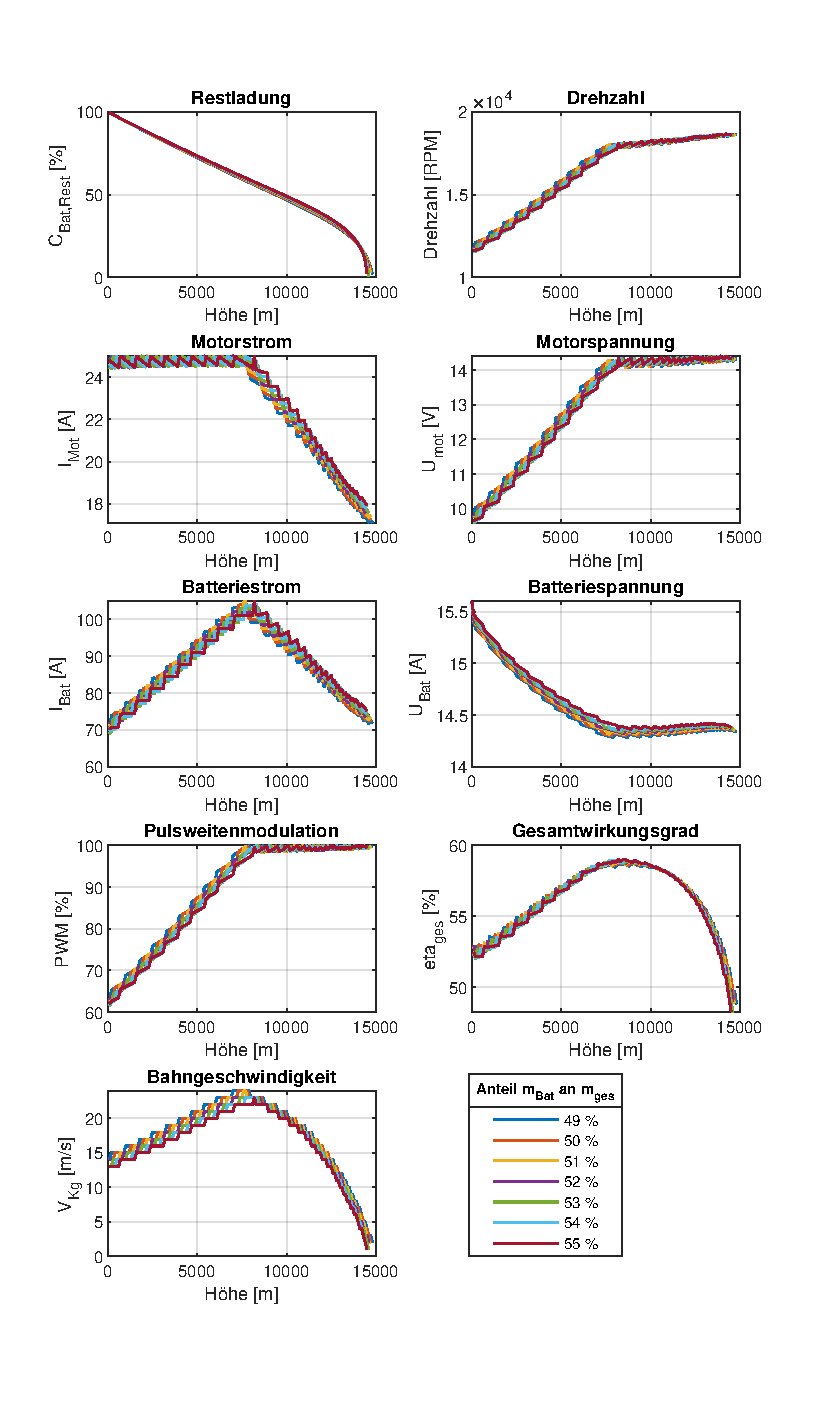
\includegraphics[scale=0.7]{Diagramme/Batteriemasse_genauer.pdf}
	\caption{genauere Untersuchung der Batteriemassenabhängigkeit (\ensuremath{m_{Mot}=\SI{106}{g}}, \ensuremath{K_V=\SI{1390}{RPM/V}}, \ensuremath{n_{Prop}=4}, \ensuremath{Propeller=\SI{10x3}{}}, \ensuremath{n_{Bat,cell}=4}, \ensuremath{u_{Wg}=\SI{10}{m/s}})}
	\label{abb:batteriemasse_genauer}
\end{figure}




\section{Verstellpropeller}
\label{sec:vprop_vorgehen}
\begin{center}
\begin{figure}[H]
\begin{struktogramm}(163,160)
\assign[1]{Multicopter- und Umgebungsparameter festlegen (im Startskript)}
\assign[1]{Diskretisierungen (Geschwindigkeit, Höhe) festlegen}
\assign[1]{Aufruf des Hauptskripts: Leistungsberechnung starten}
\while[5]{Für alle Zeilen der APC-Datenbank}
	\ifthenelse[10]{1}{1}{Stimmt Durchmesser mit dem gesuchten überein?}{ja}{nein}
		\assign[2]{Gehe zur nächsten Zeile}
		\change
		\assign[2]{Lösche Zeile}
	\ifend
\whileend
\while[5]{Für alle Propeller}
	\assign[2]{Extrahiere Propellerkennfeld}
	\assign[2]{Speicher das Ergebnis unter fortlaufenden Nummern}
	\assign[2]{Erhöhe Propellerzähler}
\whileend
\assign[1]{Initialisierung der Parameterberechnung}
\while[5]{F\"ur alle Höhenabschnitte}
	\assign[1]{H\"ohe, Dichte, Luftdruck Temperatur berechnen}
	\assign[1]{arithmetische Mittelwert berechnen}
	\assign[1]{Schub- und Leistungskennfeld anpassen}
	\assign[2]{Initialisierung der Leistungsberechnung}
	\while[5]{Für alle Bahngeschwindigkeiten}
		\assign[2]{Initialisierungen}
		\while[5]{Für alle Propeller}
			\assign[2]{\texttt{\textbf{Leistungsberechnung}}}
			\assign[2]{Berechnung benötigter Energiemenge bei dieser Bahngeschwindigkeit mit diesem Propeller}
		\whileend
		\ifthenelse[10]{4}{1}{Sind die Werte NaN?}{nein}{ja}
			\while[5]{Solange Abbruchkriterium nicht erreicht}		
				\assign[2]{Finde den Index mit der geringsten verbrauchten Energiemenge}
				\ifthenelse[10]{1}{1}{Werte innerhalb Leistungsgrenzen?}{ja}{nein}
				\assign[2]{Verlasse Schleife}
				\change
				\assign[2]{Suche nächst kleinere Energiemenge}
				\ifend
			\whileend
			\assign[2]{Übergabe aller Leistungsparameter mit diesem Index}
			\change
			\assign[2]{Verwerfe alle Ergebnisse}
		\ifend
		\assign[2]{Berechne benötigte Energie für Steiggeschwindigkeit}
	\whileend
	\ifthenelse[10]{4}{1}{Sind die Werte NaN?}{nein}{ja}
		\while[5]{Solange Abbruchkriterium nicht erreicht}		
			\assign[2]{Finde den Index mit der geringsten verbrauchten Energiemenge}
			\ifthenelse[10]{1}{1}{Werte innerhalb Leistungsgrenzen?}{ja}{nein}
			\assign[2]{Verlasse Schleife}
			\change
			\assign[2]{Suche nächst kleinere Energiemenge}
			\ifend
		\whileend
		\assign[2]{Übergabe aller Leistungsparameter mit diesem Index}
		\change
		\assign[2]{Verwerfe alle Ergebnisse}
	\ifend
	\assign[2]{Erhöhe Zählervariable}
\whileend
\assign[2]{Ergebnisse der Leistungsparameter in Diagrammen speichern}
\assign[2]{Speichern der Diagramme in .pdf-Datei}
\end{struktogramm}
\caption{Programmstruktur die Untersuchung des Nutzens eines Verstellpropellers}
\label{abb:vpp}
\end{figure}
\end{center}

Der Verlauf des Gesamtwirkungsgrades folgt eindeutig dem Verlauf des Propellerwirkungsgrades. Dieser ist die Ursache für den höheren Gesamtwirkungsgrad des Verstellpropellers (Vgl. Abb. \ref{abb:verstellprop_eta})


hier nur Wirkungsgrad
\begin{figure}[H]
\centering
	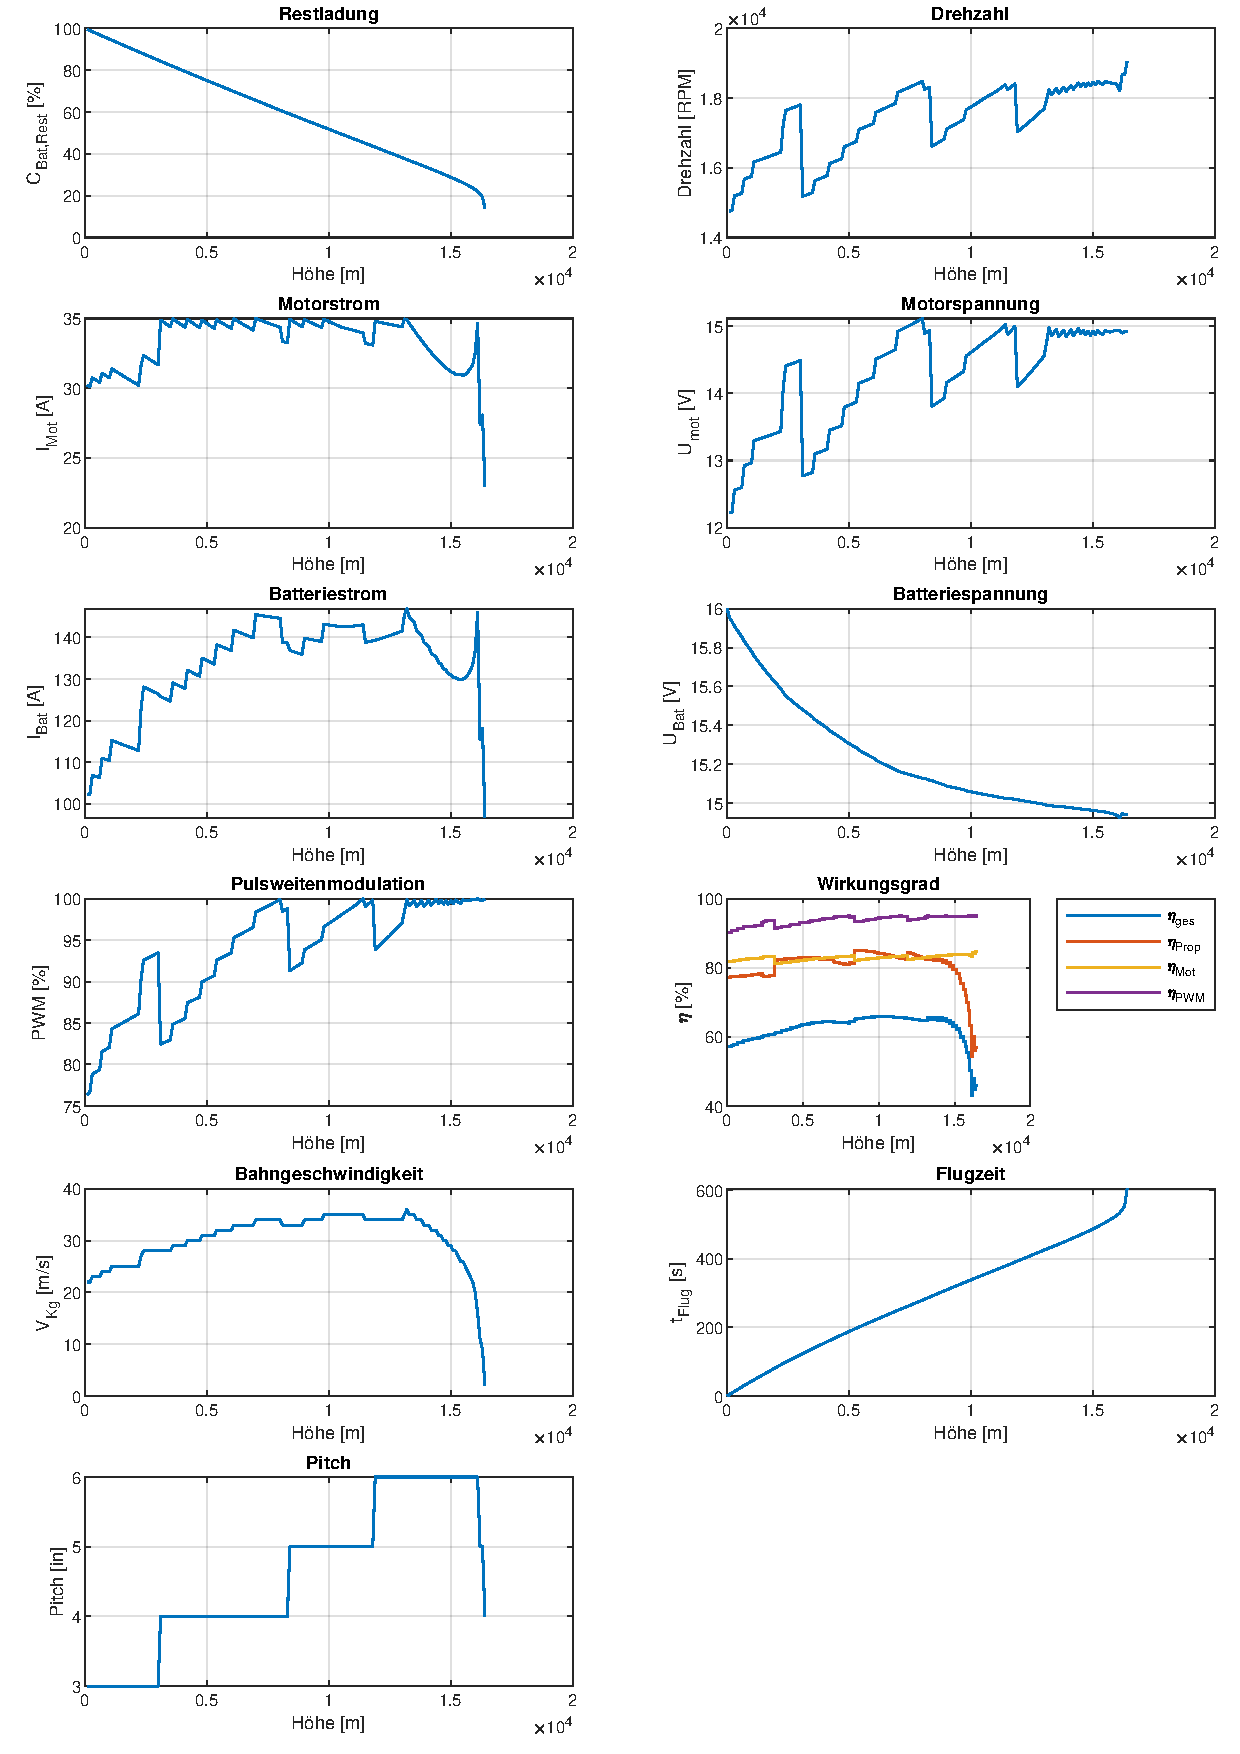
\includegraphics[scale=0.7]{Diagramme/Verstellprop_eta.pdf}
	\caption{Einfluss des Verstellpropellers auf die maximal erreichbare Höhe mit besonderem Hinblick auf die Einzelwirkungsgrade}
	\label{abb:verstellprop_eta}
\end{figure}

\begin{figure}[H]
\centering
	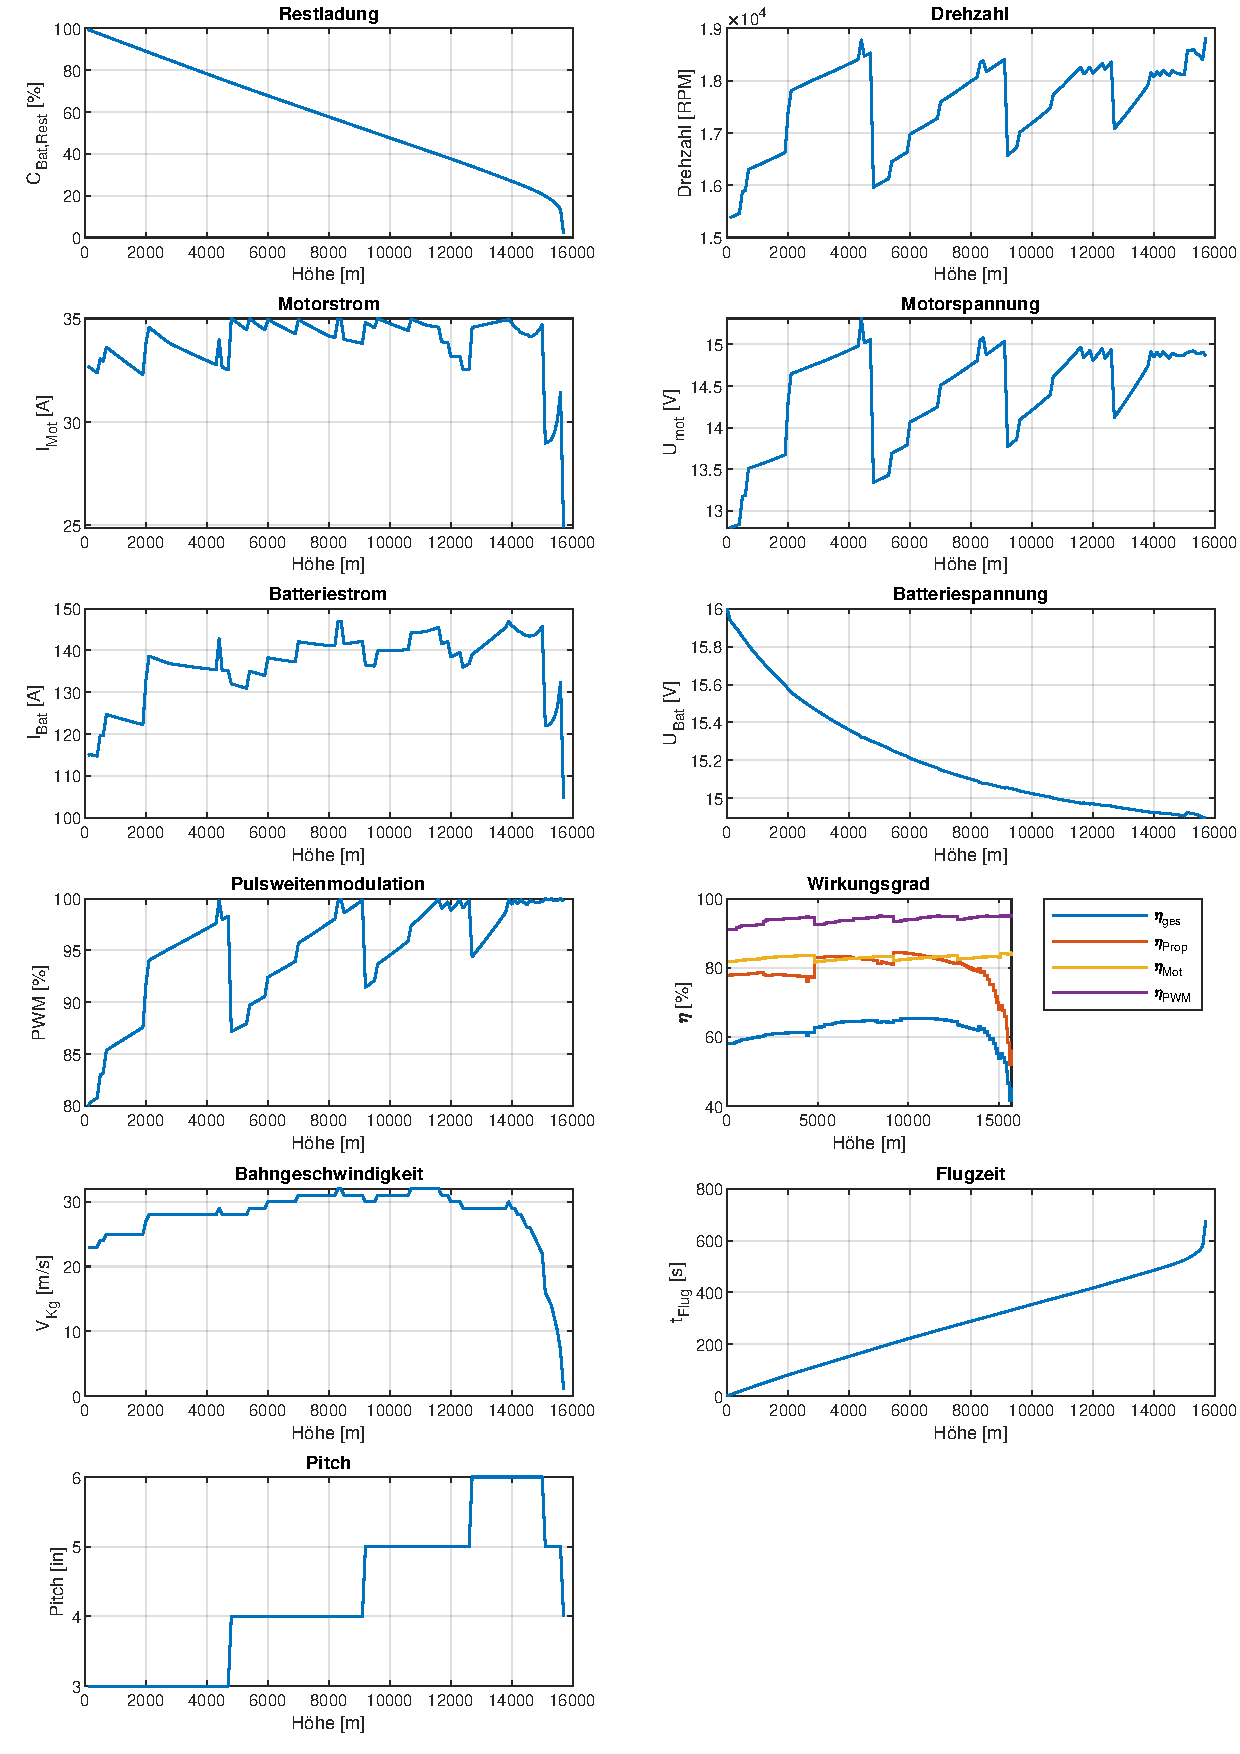
\includegraphics[scale=0.7]{Diagramme/Verstellprop_real.pdf}
	\caption{Einfluss des Verstellpropellers auf die maximal erreichbare Höhe mit einem Verstellmechanismusgewicht von 75g pro Propeller}
	\label{abb:verstellprop_real}
\end{figure}


\section{Getriebe}
\label{sec:getriebe_vorgehen}
\begin{center}
\begin{figure}[H]
\begin{struktogramm}(163,210)
\assign[1]{Multicopter- und Umgebungsparameter festlegen (im Startskript)}
\assign[1]{Diskretisierungen (Getriebe, Geschwindigkeit, Höhe) festlegen}
\assign[1]{Aufruf des Hauptskripts: Leistungsberechnung starten}
\assign[1]{Initialisierung der Parameterberechnung}
\while[5]{F\"ur alle Höhenabschnitte}
	\assign[1]{H\"ohe, Dichte, Luftdruck Temperatur berechnen}
	\assign[1]{arithmetische Mittelwert berechnen}
	\assign[1]{Schub- und Leistungskennfeld anpassen}
	\assign[2]{Initialisierung der Leistungsberechnung}
	\while[5]{Für alle Bahngeschwindigkeiten}
		\assign[2]{Initialisierungen}
		\while[5]{Für alle Übersetzungen}
			\assign[2]{\textbf{Leistungsberechnung}}
		\whileend
		\ifthenelse[10]{4}{1}{Sind die Werte NaN?}{nein}{ja}
			\while[5]{Solange Abbruchkriterium nicht erreicht}		
				\assign[2]{Finde den Index mit der geringsten verbrauchten Energiemenge}
				\ifthenelse[10]{1}{1}{Werte innerhalb Leistungsgrenzen?}{ja}{nein}
				\assign[2]{Verlasse Schleife}
				\change
				\assign[2]{Suche nächst kleineren Energiemenge}
				\ifend
			\whileend
			\assign[2]{Übergabe aller Leistungsparameter mit diesem Index}
			\change
			\assign[2]{Verwerfe alle Ergebnisse}
		\ifend
		\assign[2]{Berechne benötigte Energie für Steiggeschwindigkeit}
	\whileend
	\ifthenelse[10]{4}{1}{Sind die Werte NaN?}{nein}{ja}
		\while[5]{Solange Abbruchkriterium nicht erreicht}		
			\assign[2]{Finde den Index mit der geringsten verbrauchten Energiemenge}
			\ifthenelse[10]{1}{1}{Werte innerhalb Leistungsgrenzen?}{ja}{nein}
			\assign[2]{Verlasse Schleife}
			\change
			\assign[2]{Suche nächst kleinere Energiemenge}
			\ifend
		\whileend
		\assign[2]{Übergabe aller Leistungsparameter mit diesem Index}
		\change
		\assign[2]{Verwerfe alle Ergebnisse}
	\ifend
	\assign[2]{Erhöhe Zählervariable}
\whileend
\assign[2]{Ergebnisse der Leistungsparameter in Diagrammen speichern}
\assign[2]{Speichern der Diagramme in .pdf-Datei}
\end{struktogramm}
\caption{Programmstruktur die Untersuchung des Nutzens eines Getriebes}
\label{abb:getriebe}
\end{figure}
\end{center}

\begin{figure}[H]
\centering
	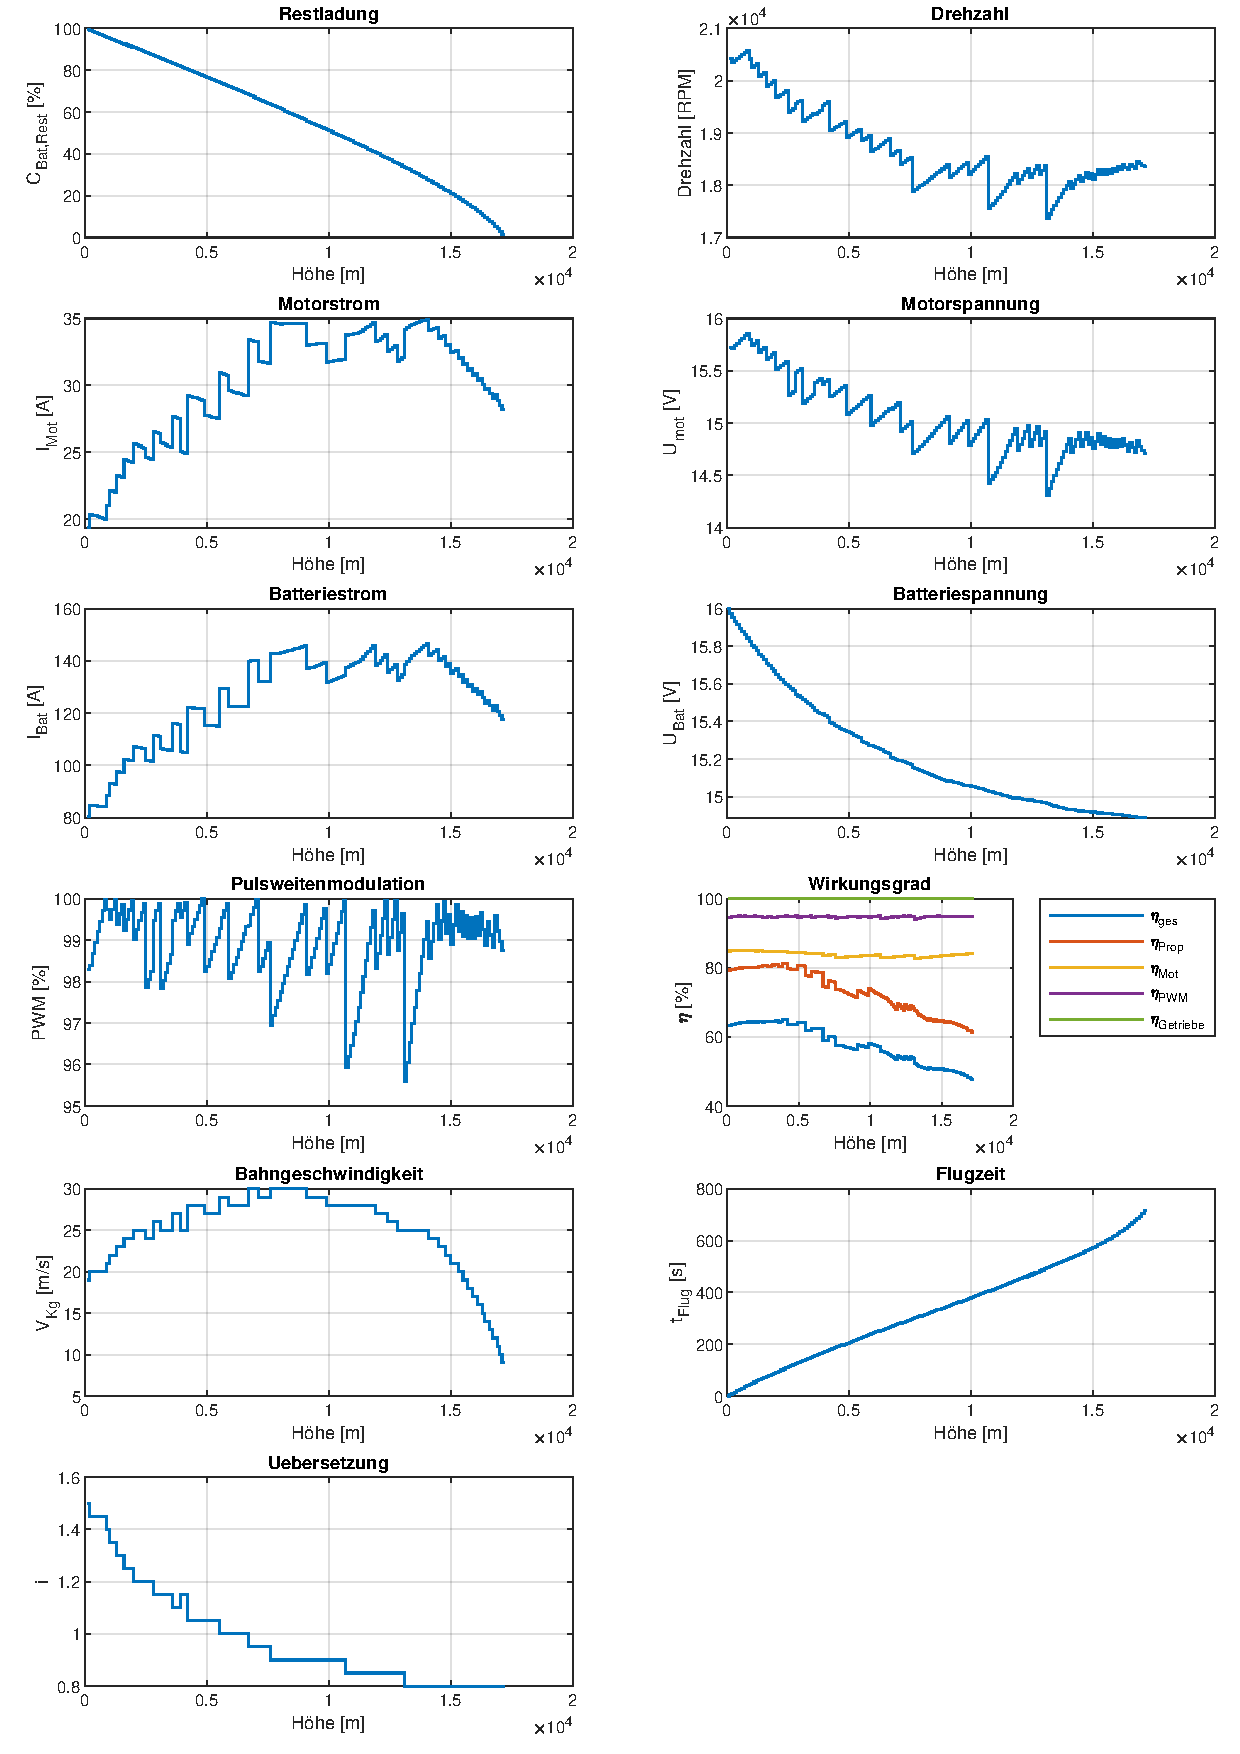
\includegraphics[scale=0.7]{Diagramme/Getriebe_wirkungsgrade.pdf}
	\caption{Einfluss eines Getriebes auf die maximal erreichbare Höhe mit besonderem Hinblick auf die Einzelwirkungsgrade}
	\label{abb:getriebe_wirkungsgrade}
\end{figure}

\missingfigure{realistische Werte, keine rosarote Brille}

\missingfigure{anderer Motor mit anderem KV}

\begin{figure}[H]
\centering
	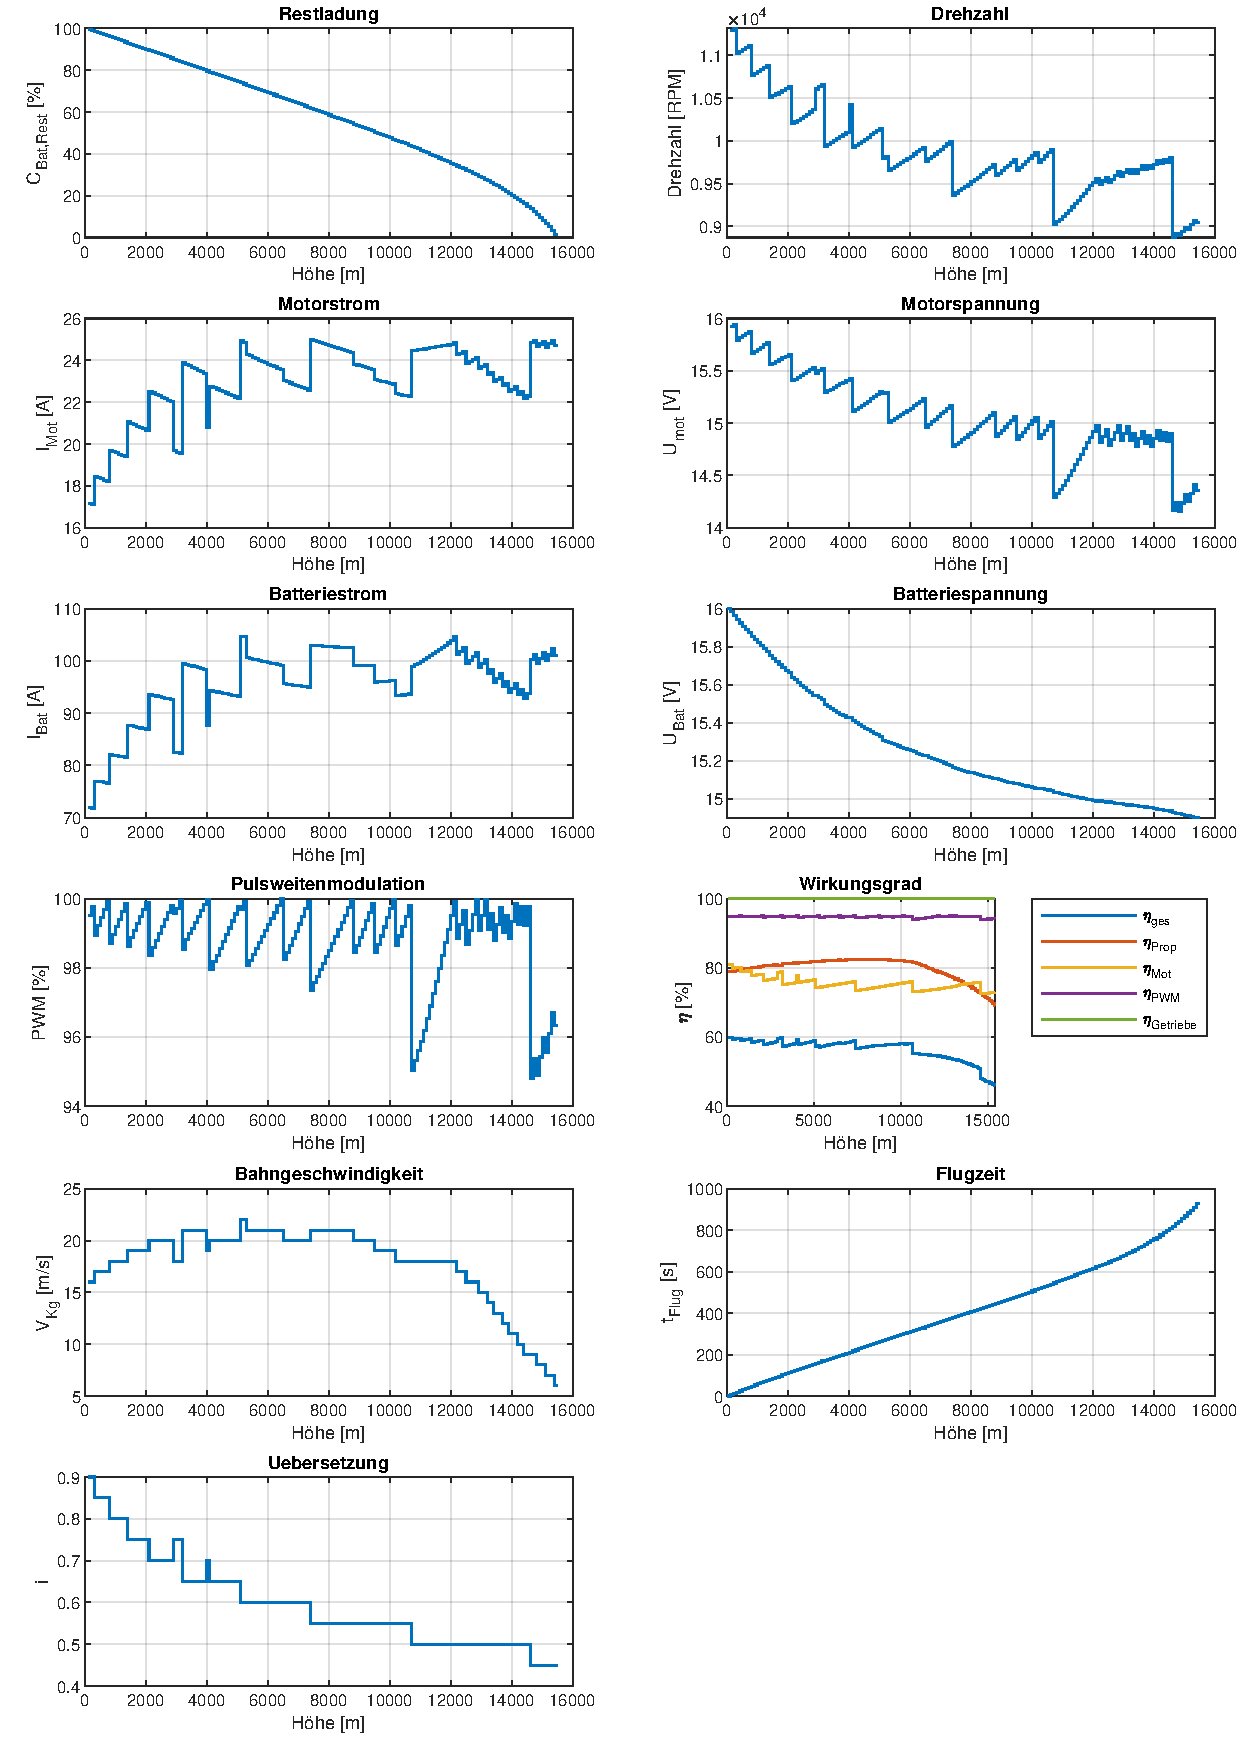
\includegraphics[scale=0.7]{Diagramme/Getriebe_KV.pdf}
	\caption{Einfluss des Motors in Kombination eines Getriebes auf die maximal erreichbare Höhe}
	\label{abb:getriebe_wirkungsgrade}
\end{figure}
\begin{figure}[H]
\centering
	\includegraphics[scale=0.7]{Diagramme/Dud_KV.pdf}
	\caption{Übersetzung für ein Getriebe}
	\label{abb:getriebe_wirkungsgrade}
\end{figure}

\end{appendix}
